% Options for packages loaded elsewhere
\PassOptionsToPackage{unicode}{hyperref}
\PassOptionsToPackage{hyphens}{url}
\PassOptionsToPackage{dvipsnames,svgnames,x11names}{xcolor}
%
\documentclass[
  letterpaper,
  DIV=11,
  numbers=noendperiod]{scrartcl}

\usepackage{amsmath,amssymb}
\usepackage{iftex}
\ifPDFTeX
  \usepackage[T1]{fontenc}
  \usepackage[utf8]{inputenc}
  \usepackage{textcomp} % provide euro and other symbols
\else % if luatex or xetex
  \usepackage{unicode-math}
  \defaultfontfeatures{Scale=MatchLowercase}
  \defaultfontfeatures[\rmfamily]{Ligatures=TeX,Scale=1}
\fi
\usepackage{lmodern}
\ifPDFTeX\else  
    % xetex/luatex font selection
\fi
% Use upquote if available, for straight quotes in verbatim environments
\IfFileExists{upquote.sty}{\usepackage{upquote}}{}
\IfFileExists{microtype.sty}{% use microtype if available
  \usepackage[]{microtype}
  \UseMicrotypeSet[protrusion]{basicmath} % disable protrusion for tt fonts
}{}
\makeatletter
\@ifundefined{KOMAClassName}{% if non-KOMA class
  \IfFileExists{parskip.sty}{%
    \usepackage{parskip}
  }{% else
    \setlength{\parindent}{0pt}
    \setlength{\parskip}{6pt plus 2pt minus 1pt}}
}{% if KOMA class
  \KOMAoptions{parskip=half}}
\makeatother
\usepackage{xcolor}
\setlength{\emergencystretch}{3em} % prevent overfull lines
\setcounter{secnumdepth}{-\maxdimen} % remove section numbering
% Make \paragraph and \subparagraph free-standing
\makeatletter
\ifx\paragraph\undefined\else
  \let\oldparagraph\paragraph
  \renewcommand{\paragraph}{
    \@ifstar
      \xxxParagraphStar
      \xxxParagraphNoStar
  }
  \newcommand{\xxxParagraphStar}[1]{\oldparagraph*{#1}\mbox{}}
  \newcommand{\xxxParagraphNoStar}[1]{\oldparagraph{#1}\mbox{}}
\fi
\ifx\subparagraph\undefined\else
  \let\oldsubparagraph\subparagraph
  \renewcommand{\subparagraph}{
    \@ifstar
      \xxxSubParagraphStar
      \xxxSubParagraphNoStar
  }
  \newcommand{\xxxSubParagraphStar}[1]{\oldsubparagraph*{#1}\mbox{}}
  \newcommand{\xxxSubParagraphNoStar}[1]{\oldsubparagraph{#1}\mbox{}}
\fi
\makeatother

\usepackage{color}
\usepackage{fancyvrb}
\newcommand{\VerbBar}{|}
\newcommand{\VERB}{\Verb[commandchars=\\\{\}]}
\DefineVerbatimEnvironment{Highlighting}{Verbatim}{commandchars=\\\{\}}
% Add ',fontsize=\small' for more characters per line
\usepackage{framed}
\definecolor{shadecolor}{RGB}{241,243,245}
\newenvironment{Shaded}{\begin{snugshade}}{\end{snugshade}}
\newcommand{\AlertTok}[1]{\textcolor[rgb]{0.68,0.00,0.00}{#1}}
\newcommand{\AnnotationTok}[1]{\textcolor[rgb]{0.37,0.37,0.37}{#1}}
\newcommand{\AttributeTok}[1]{\textcolor[rgb]{0.40,0.45,0.13}{#1}}
\newcommand{\BaseNTok}[1]{\textcolor[rgb]{0.68,0.00,0.00}{#1}}
\newcommand{\BuiltInTok}[1]{\textcolor[rgb]{0.00,0.23,0.31}{#1}}
\newcommand{\CharTok}[1]{\textcolor[rgb]{0.13,0.47,0.30}{#1}}
\newcommand{\CommentTok}[1]{\textcolor[rgb]{0.37,0.37,0.37}{#1}}
\newcommand{\CommentVarTok}[1]{\textcolor[rgb]{0.37,0.37,0.37}{\textit{#1}}}
\newcommand{\ConstantTok}[1]{\textcolor[rgb]{0.56,0.35,0.01}{#1}}
\newcommand{\ControlFlowTok}[1]{\textcolor[rgb]{0.00,0.23,0.31}{\textbf{#1}}}
\newcommand{\DataTypeTok}[1]{\textcolor[rgb]{0.68,0.00,0.00}{#1}}
\newcommand{\DecValTok}[1]{\textcolor[rgb]{0.68,0.00,0.00}{#1}}
\newcommand{\DocumentationTok}[1]{\textcolor[rgb]{0.37,0.37,0.37}{\textit{#1}}}
\newcommand{\ErrorTok}[1]{\textcolor[rgb]{0.68,0.00,0.00}{#1}}
\newcommand{\ExtensionTok}[1]{\textcolor[rgb]{0.00,0.23,0.31}{#1}}
\newcommand{\FloatTok}[1]{\textcolor[rgb]{0.68,0.00,0.00}{#1}}
\newcommand{\FunctionTok}[1]{\textcolor[rgb]{0.28,0.35,0.67}{#1}}
\newcommand{\ImportTok}[1]{\textcolor[rgb]{0.00,0.46,0.62}{#1}}
\newcommand{\InformationTok}[1]{\textcolor[rgb]{0.37,0.37,0.37}{#1}}
\newcommand{\KeywordTok}[1]{\textcolor[rgb]{0.00,0.23,0.31}{\textbf{#1}}}
\newcommand{\NormalTok}[1]{\textcolor[rgb]{0.00,0.23,0.31}{#1}}
\newcommand{\OperatorTok}[1]{\textcolor[rgb]{0.37,0.37,0.37}{#1}}
\newcommand{\OtherTok}[1]{\textcolor[rgb]{0.00,0.23,0.31}{#1}}
\newcommand{\PreprocessorTok}[1]{\textcolor[rgb]{0.68,0.00,0.00}{#1}}
\newcommand{\RegionMarkerTok}[1]{\textcolor[rgb]{0.00,0.23,0.31}{#1}}
\newcommand{\SpecialCharTok}[1]{\textcolor[rgb]{0.37,0.37,0.37}{#1}}
\newcommand{\SpecialStringTok}[1]{\textcolor[rgb]{0.13,0.47,0.30}{#1}}
\newcommand{\StringTok}[1]{\textcolor[rgb]{0.13,0.47,0.30}{#1}}
\newcommand{\VariableTok}[1]{\textcolor[rgb]{0.07,0.07,0.07}{#1}}
\newcommand{\VerbatimStringTok}[1]{\textcolor[rgb]{0.13,0.47,0.30}{#1}}
\newcommand{\WarningTok}[1]{\textcolor[rgb]{0.37,0.37,0.37}{\textit{#1}}}

\providecommand{\tightlist}{%
  \setlength{\itemsep}{0pt}\setlength{\parskip}{0pt}}\usepackage{longtable,booktabs,array}
\usepackage{calc} % for calculating minipage widths
% Correct order of tables after \paragraph or \subparagraph
\usepackage{etoolbox}
\makeatletter
\patchcmd\longtable{\par}{\if@noskipsec\mbox{}\fi\par}{}{}
\makeatother
% Allow footnotes in longtable head/foot
\IfFileExists{footnotehyper.sty}{\usepackage{footnotehyper}}{\usepackage{footnote}}
\makesavenoteenv{longtable}
\usepackage{graphicx}
\makeatletter
\newsavebox\pandoc@box
\newcommand*\pandocbounded[1]{% scales image to fit in text height/width
  \sbox\pandoc@box{#1}%
  \Gscale@div\@tempa{\textheight}{\dimexpr\ht\pandoc@box+\dp\pandoc@box\relax}%
  \Gscale@div\@tempb{\linewidth}{\wd\pandoc@box}%
  \ifdim\@tempb\p@<\@tempa\p@\let\@tempa\@tempb\fi% select the smaller of both
  \ifdim\@tempa\p@<\p@\scalebox{\@tempa}{\usebox\pandoc@box}%
  \else\usebox{\pandoc@box}%
  \fi%
}
% Set default figure placement to htbp
\def\fps@figure{htbp}
\makeatother

\usepackage{fvextra}
\DefineVerbatimEnvironment{Highlighting}{Verbatim}{breaklines,commandchars=\\\{\}}
\KOMAoption{captions}{tableheading}
\makeatletter
\@ifpackageloaded{caption}{}{\usepackage{caption}}
\AtBeginDocument{%
\ifdefined\contentsname
  \renewcommand*\contentsname{Table of contents}
\else
  \newcommand\contentsname{Table of contents}
\fi
\ifdefined\listfigurename
  \renewcommand*\listfigurename{List of Figures}
\else
  \newcommand\listfigurename{List of Figures}
\fi
\ifdefined\listtablename
  \renewcommand*\listtablename{List of Tables}
\else
  \newcommand\listtablename{List of Tables}
\fi
\ifdefined\figurename
  \renewcommand*\figurename{Figure}
\else
  \newcommand\figurename{Figure}
\fi
\ifdefined\tablename
  \renewcommand*\tablename{Table}
\else
  \newcommand\tablename{Table}
\fi
}
\@ifpackageloaded{float}{}{\usepackage{float}}
\floatstyle{ruled}
\@ifundefined{c@chapter}{\newfloat{codelisting}{h}{lop}}{\newfloat{codelisting}{h}{lop}[chapter]}
\floatname{codelisting}{Listing}
\newcommand*\listoflistings{\listof{codelisting}{List of Listings}}
\makeatother
\makeatletter
\makeatother
\makeatletter
\@ifpackageloaded{caption}{}{\usepackage{caption}}
\@ifpackageloaded{subcaption}{}{\usepackage{subcaption}}
\makeatother

\usepackage{bookmark}

\IfFileExists{xurl.sty}{\usepackage{xurl}}{} % add URL line breaks if available
\urlstyle{same} % disable monospaced font for URLs
\hypersetup{
  pdftitle={Problem Set 4\_Yuki\_Tianhao},
  colorlinks=true,
  linkcolor={blue},
  filecolor={Maroon},
  citecolor={Blue},
  urlcolor={Blue},
  pdfcreator={LaTeX via pandoc}}


\title{Problem Set 4\_Yuki\_Tianhao}
\author{}
\date{}

\begin{document}
\maketitle

\RecustomVerbatimEnvironment{verbatim}{Verbatim}{
  showspaces = false,
  showtabs = false,
  breaksymbolleft={},
  breaklines
}


\textbf{PS4:} Due Sat Nov 2 at 5:00PM Central. Worth 100 points. We use
(\texttt{*}) to indicate a problem that we think might be time
consuming.

\subsection{Style Points (10 pts)}\label{style-points-10-pts}

Please refer to the minilesson on code style
\textbf{\href{https://uchicago.zoom.us/rec/share/pG_wQ-pHTQrJTmqNn4rcrw5V194M2H2s-2jdy8oVhWHkd_yZt9o162IWurpA-fxU.BIQlSgZLRYctvzp-}{here}}.

\subsection{Submission Steps (10 pts)}\label{submission-steps-10-pts}

\begin{enumerate}
\def\labelenumi{\arabic{enumi}.}
\tightlist
\item
  This problem set is a paired problem set.
\item
  Play paper, scissors, rock to determine who goes first. Call that
  person \emph{Partner 1}.

  \begin{itemize}
  \tightlist
  \item
    Partner 1 (name and cnet ID): Yuki Yan \& yukiyan
  \item
    Partner 2 (name and cnet ID): Tianhao Zhang \& tz2205
  \end{itemize}
\item
  Partner 1 will accept the \texttt{ps4} and then share the link it
  creates with their partner. You can only share it with one partner so
  you will not be able to change it after your partner has accepted.
\item
  ``This submission is our work alone and complies with the 30538
  integrity policy.'' Add your initials to indicate your agreement:
  **YY** **TZ**
\item
  ``I have uploaded the names of anyone else other than my partner and I
  worked with on the problem set
  \textbf{\href{https://docs.google.com/forms/d/185usrCREQaUbvAXpWhChkjghdGgmAZXA3lPWpXLLsts/edit}{here}}''
  (1 point)
\item
  Late coins used this pset: **\textbackslash1\_** Late coins left after
  submission: **\textbackslash1\_**
\item
  Knit your \texttt{ps4.qmd} to an PDF file to make \texttt{ps4.pdf},

  \begin{itemize}
  \tightlist
  \item
    The PDF should not be more than 25 pages. Use \texttt{head()} and
    re-size figures when appropriate.
  \end{itemize}
\item
  (Partner 1): push \texttt{ps4.qmd} and \texttt{ps4.pdf} to your github
  repo.
\item
  (Partner 1): submit \texttt{ps4.pdf} via Gradescope. Add your partner
  on Gradescope.
\item
  (Partner 1): tag your submission in Gradescope
\end{enumerate}

\textbf{Important:} Repositories are for tracking code. \textbf{Do not
commit the data or shapefiles to your repo.} The best way to do this is
with \texttt{.gitignore}, which we have covered in class. If you do
accidentally commit the data, Github has a
\href{https://docs.github.com/en/repositories/working-with-files/managing-large-files/about-large-files-on-github\#removing-files-from-a-repositorys-history}{guide}.
The best course of action depends on whether you have pushed yet. This
also means that both partners will have to download the initial raw data
and any data cleaning code will need to be re-run on both partners'
computers.

\subsection{Download and explore the Provider of Services (POS) file (10
pts)}\label{download-and-explore-the-provider-of-services-pos-file-10-pts}

\begin{enumerate}
\def\labelenumi{\arabic{enumi}.}
\item
  PRVDR\_CTGRY\_SBTYP\_CD - Provider Category Subtype Code
  PRVDR\_CTGRY\_CD - Provider Category Code PRVDR\_NUM - CMS
  Certification Number PGM\_TRMNTN\_CD - current termination status
  CITY\_NAME - City where the facility is located STATE\_CD - State code
  ZIP\_CD - Zip code of the facility FAC\_NAME - Facility name ST\_ADR -
  Street address PRVDR\_NUM - Provider Number
\item
  \begin{enumerate}
  \def\labelenumii{\alph{enumii}.}
  \tightlist
  \item
  \end{enumerate}
\end{enumerate}

\begin{Shaded}
\begin{Highlighting}[]
\ImportTok{import}\NormalTok{ warnings}
\NormalTok{warnings.filterwarnings(}\StringTok{"ignore"}\NormalTok{)}
\ImportTok{import}\NormalTok{ pandas }\ImportTok{as}\NormalTok{ pd}
\ImportTok{import}\NormalTok{ matplotlib.pyplot }\ImportTok{as}\NormalTok{ plt}


\KeywordTok{def}\NormalTok{ load\_and\_filter\_pos(file\_path, year):}
\NormalTok{    pos\_data }\OperatorTok{=}\NormalTok{ pd.read\_csv(file\_path, low\_memory}\OperatorTok{=}\VariableTok{False}\NormalTok{, encoding}\OperatorTok{=}\StringTok{\textquotesingle{}latin1\textquotesingle{}}\NormalTok{)}
    
\NormalTok{    short\_term\_hospitals }\OperatorTok{=}\NormalTok{ pos\_data[(pos\_data[}\StringTok{\textquotesingle{}PRVDR\_CTGRY\_CD\textquotesingle{}}\NormalTok{] }\OperatorTok{==} \DecValTok{1}\NormalTok{) }\OperatorTok{\&} 
\NormalTok{                                    (pos\_data[}\StringTok{\textquotesingle{}PRVDR\_CTGRY\_SBTYP\_CD\textquotesingle{}}\NormalTok{] }\OperatorTok{==} \DecValTok{1}\NormalTok{)]}
    
    \CommentTok{\# Add column }
\NormalTok{    short\_term\_hospitals[}\StringTok{\textquotesingle{}Year\textquotesingle{}}\NormalTok{] }\OperatorTok{=}\NormalTok{ year}
    \BuiltInTok{print}\NormalTok{(}\SpecialStringTok{f"Year }\SpecialCharTok{\{}\NormalTok{year}\SpecialCharTok{\}}\SpecialStringTok{ {-} Number of short{-}term hospitals: }\SpecialCharTok{\{}\BuiltInTok{len}\NormalTok{(short\_term\_hospitals)}\SpecialCharTok{\}}\SpecialStringTok{"}\NormalTok{)  }\CommentTok{\# Check the count}
    \ControlFlowTok{return}\NormalTok{ short\_term\_hospitals}

\NormalTok{pos2016 }\OperatorTok{=}\NormalTok{ load\_and\_filter\_pos(}\StringTok{\textquotesingle{}pos2016.csv\textquotesingle{}}\NormalTok{, }\DecValTok{2016}\NormalTok{)}
\NormalTok{pos2017 }\OperatorTok{=}\NormalTok{ load\_and\_filter\_pos(}\StringTok{\textquotesingle{}pos2017.csv\textquotesingle{}}\NormalTok{, }\DecValTok{2017}\NormalTok{)}
\NormalTok{pos2018 }\OperatorTok{=}\NormalTok{ load\_and\_filter\_pos(}\StringTok{\textquotesingle{}pos2018.csv\textquotesingle{}}\NormalTok{, }\DecValTok{2018}\NormalTok{)}
\NormalTok{pos2019 }\OperatorTok{=}\NormalTok{ load\_and\_filter\_pos(}\StringTok{\textquotesingle{}pos2019.csv\textquotesingle{}}\NormalTok{, }\DecValTok{2019}\NormalTok{)}

\NormalTok{all\_years\_data }\OperatorTok{=}\NormalTok{ pd.concat([pos2016, pos2017, pos2018, pos2019], ignore\_index}\OperatorTok{=}\VariableTok{True}\NormalTok{)}

\NormalTok{observations\_by\_year }\OperatorTok{=}\NormalTok{ all\_years\_data[}\StringTok{\textquotesingle{}Year\textquotesingle{}}\NormalTok{].value\_counts().sort\_index()}

\CommentTok{\# Plot }
\NormalTok{plt.figure(figsize}\OperatorTok{=}\NormalTok{(}\DecValTok{10}\NormalTok{, }\DecValTok{6}\NormalTok{))}
\NormalTok{observations\_by\_year.plot(kind}\OperatorTok{=}\StringTok{\textquotesingle{}bar\textquotesingle{}}\NormalTok{)}
\NormalTok{plt.title(}\StringTok{\textquotesingle{}Number of Short{-}Term Hospital Observations by Year\textquotesingle{}}\NormalTok{)}
\NormalTok{plt.xlabel(}\StringTok{\textquotesingle{}Year\textquotesingle{}}\NormalTok{)}
\NormalTok{plt.ylabel(}\StringTok{\textquotesingle{}Number of Observations\textquotesingle{}}\NormalTok{)}
\NormalTok{plt.ylim(}\DecValTok{7240}\NormalTok{, }\DecValTok{7305}\NormalTok{)}
\NormalTok{plt.yticks(}\BuiltInTok{range}\NormalTok{(}\DecValTok{7240}\NormalTok{, }\DecValTok{7306}\NormalTok{, }\DecValTok{5}\NormalTok{))}

\CommentTok{\# y{-}axis}
\NormalTok{plt.yticks(}\BuiltInTok{range}\NormalTok{(}\BuiltInTok{min}\NormalTok{(observations\_by\_year) }\OperatorTok{{-}} \DecValTok{10}\NormalTok{, }\BuiltInTok{max}\NormalTok{(observations\_by\_year) }\OperatorTok{+} \DecValTok{10}\NormalTok{, }\DecValTok{10}\NormalTok{))}

\NormalTok{plt.xticks(rotation}\OperatorTok{=}\DecValTok{0}\NormalTok{)}
\NormalTok{plt.show()}
\end{Highlighting}
\end{Shaded}

\begin{verbatim}
Year 2016 - Number of short-term hospitals: 7245
Year 2017 - Number of short-term hospitals: 7260
Year 2018 - Number of short-term hospitals: 7277
Year 2019 - Number of short-term hospitals: 7303
\end{verbatim}

\pandocbounded{\includegraphics[keepaspectratio]{pset4_template_files/figure-pdf/cell-2-output-2.pdf}}

\begin{enumerate}
\def\labelenumi{\arabic{enumi}.}
\setcounter{enumi}{3}
\tightlist
\item
  \begin{enumerate}
  \def\labelenumii{\alph{enumii}.}
  \tightlist
  \item
  \end{enumerate}
\end{enumerate}

\begin{Shaded}
\begin{Highlighting}[]
\ImportTok{import}\NormalTok{ pandas }\ImportTok{as}\NormalTok{ pd}
\ImportTok{import}\NormalTok{ matplotlib.pyplot }\ImportTok{as}\NormalTok{ plt}

\NormalTok{unique\_hospitals\_by\_year }\OperatorTok{=}\NormalTok{ all\_years\_data.groupby(}\StringTok{\textquotesingle{}Year\textquotesingle{}}\NormalTok{)[}\StringTok{\textquotesingle{}PRVDR\_NUM\textquotesingle{}}\NormalTok{].nunique()}

\CommentTok{\# Plot the number of unique hospitals per year}
\NormalTok{plt.figure(figsize}\OperatorTok{=}\NormalTok{(}\DecValTok{10}\NormalTok{, }\DecValTok{6}\NormalTok{))}
\NormalTok{unique\_hospitals\_by\_year.plot(kind}\OperatorTok{=}\StringTok{\textquotesingle{}bar\textquotesingle{}}\NormalTok{)}
\NormalTok{plt.title(}\StringTok{\textquotesingle{}Number of Unique Short{-}Term Hospitals by Year\textquotesingle{}}\NormalTok{)}
\NormalTok{plt.xlabel(}\StringTok{\textquotesingle{}Year\textquotesingle{}}\NormalTok{)}
\NormalTok{plt.ylabel(}\StringTok{\textquotesingle{}Number of Unique Hospitals\textquotesingle{}}\NormalTok{)}
\NormalTok{plt.ylim(}\DecValTok{7240}\NormalTok{, }\DecValTok{7305}\NormalTok{)  }\CommentTok{\# Set a similar y{-}axis range for easy comparison}
\NormalTok{plt.xticks(rotation}\OperatorTok{=}\DecValTok{0}\NormalTok{)}
\NormalTok{plt.show()}

\CommentTok{\# Display the count for reference}
\BuiltInTok{print}\NormalTok{(unique\_hospitals\_by\_year)}
\end{Highlighting}
\end{Shaded}

\pandocbounded{\includegraphics[keepaspectratio]{pset4_template_files/figure-pdf/cell-3-output-1.pdf}}

\begin{verbatim}
Year
2016    7245
2017    7260
2018    7277
2019    7303
Name: PRVDR_NUM, dtype: int64
\end{verbatim}

\begin{verbatim}
b.
Each CMS certification number (PRVDR_NUM) appears only once per year. This indicates that the dataset is structured so that each hospital has a single, unique record in each year, without duplicate entries or multiple records reflecting different operational statuses or characteristics within the same year. Since there are no duplicates within each year, the dataset is reliable for examining trends over time, such as changes in the number of active short-term hospitals each year. The increase in counts from 2016 to 2019 reflects an actual trend rather than potential data artifacts caused by duplicated records.
\end{verbatim}

\subsection{Identify hospital closures in POS file (15 pts)
(*)}\label{identify-hospital-closures-in-pos-file-15-pts}

\begin{enumerate}
\def\labelenumi{\arabic{enumi}.}
\tightlist
\item
\end{enumerate}

\begin{Shaded}
\begin{Highlighting}[]
\KeywordTok{def}\NormalTok{ load\_and\_filter\_pos(file\_path, year):}
\NormalTok{    pos\_data }\OperatorTok{=}\NormalTok{ pd.read\_csv(file\_path, low\_memory}\OperatorTok{=}\VariableTok{False}\NormalTok{, encoding}\OperatorTok{=}\StringTok{\textquotesingle{}latin1\textquotesingle{}}\NormalTok{)}
\NormalTok{    pos\_data[}\StringTok{\textquotesingle{}Year\textquotesingle{}}\NormalTok{] }\OperatorTok{=}\NormalTok{ year}
    \ControlFlowTok{return}\NormalTok{ pos\_data}

\NormalTok{pos2016 }\OperatorTok{=}\NormalTok{ load\_and\_filter\_pos(}\StringTok{\textquotesingle{}pos2016.csv\textquotesingle{}}\NormalTok{, }\DecValTok{2016}\NormalTok{)}
\NormalTok{pos2017 }\OperatorTok{=}\NormalTok{ load\_and\_filter\_pos(}\StringTok{\textquotesingle{}pos2017.csv\textquotesingle{}}\NormalTok{, }\DecValTok{2017}\NormalTok{)}
\NormalTok{pos2018 }\OperatorTok{=}\NormalTok{ load\_and\_filter\_pos(}\StringTok{\textquotesingle{}pos2018.csv\textquotesingle{}}\NormalTok{, }\DecValTok{2018}\NormalTok{)}
\NormalTok{pos2019 }\OperatorTok{=}\NormalTok{ load\_and\_filter\_pos(}\StringTok{\textquotesingle{}pos2019.csv\textquotesingle{}}\NormalTok{, }\DecValTok{2019}\NormalTok{)}
\NormalTok{all\_years\_data }\OperatorTok{=}\NormalTok{ pd.concat([pos2016, pos2017, pos2018, pos2019], ignore\_index}\OperatorTok{=}\VariableTok{True}\NormalTok{)}
\end{Highlighting}
\end{Shaded}

\begin{Shaded}
\begin{Highlighting}[]
\NormalTok{pivoted\_data }\OperatorTok{=}\NormalTok{ all\_years\_data.pivot\_table(}
\NormalTok{    index}\OperatorTok{=}\NormalTok{[}\StringTok{\textquotesingle{}PRVDR\_NUM\textquotesingle{}}\NormalTok{, }\StringTok{\textquotesingle{}FAC\_NAME\textquotesingle{}}\NormalTok{, }\StringTok{\textquotesingle{}ZIP\_CD\textquotesingle{}}\NormalTok{], }
\NormalTok{    columns}\OperatorTok{=}\StringTok{\textquotesingle{}Year\textquotesingle{}}\NormalTok{, }
\NormalTok{    values}\OperatorTok{=}\StringTok{\textquotesingle{}PGM\_TRMNTN\_CD\textquotesingle{}}\NormalTok{, }
\NormalTok{    aggfunc}\OperatorTok{=}\StringTok{\textquotesingle{}first\textquotesingle{}}
\NormalTok{).reset\_index()}
\end{Highlighting}
\end{Shaded}

\begin{Shaded}
\begin{Highlighting}[]
\NormalTok{pivoted\_data[}\StringTok{\textquotesingle{}Suspected\_Closure\_Year\textquotesingle{}}\NormalTok{] }\OperatorTok{=}\NormalTok{ pivoted\_data.}\BuiltInTok{apply}\NormalTok{(}
    \KeywordTok{lambda}\NormalTok{ row: }\BuiltInTok{next}\NormalTok{((year }\ControlFlowTok{for}\NormalTok{ year }\KeywordTok{in}\NormalTok{ [}\DecValTok{2017}\NormalTok{, }\DecValTok{2018}\NormalTok{, }\DecValTok{2019}\NormalTok{] }\ControlFlowTok{if} \OperatorTok{\textbackslash{}}
\NormalTok{        (pd.isna(row[year]) }\KeywordTok{or}\NormalTok{ row[year] }\OperatorTok{!=} \DecValTok{0}\NormalTok{) }\KeywordTok{and}\NormalTok{ row[}\DecValTok{2016}\NormalTok{] }\OperatorTok{==} \DecValTok{0}\NormalTok{), }\VariableTok{None}\NormalTok{), axis}\OperatorTok{=}\DecValTok{1}\NormalTok{)}
\NormalTok{suspected\_closures }\OperatorTok{=}\NormalTok{ pivoted\_data.dropna(subset}\OperatorTok{=}\NormalTok{[}\StringTok{\textquotesingle{}Suspected\_Closure\_Year\textquotesingle{}}\NormalTok{])}
\end{Highlighting}
\end{Shaded}

\begin{Shaded}
\begin{Highlighting}[]
\NormalTok{suspected\_closures\_list }\OperatorTok{=}\NormalTok{ suspected\_closures[[}\StringTok{\textquotesingle{}FAC\_NAME\textquotesingle{}}\NormalTok{, }\StringTok{\textquotesingle{}ZIP\_CD\textquotesingle{}}\NormalTok{, }\StringTok{\textquotesingle{}Suspected\_Closure\_Year\textquotesingle{}}\NormalTok{]]}
\NormalTok{total\_suspected\_closures }\OperatorTok{=} \BuiltInTok{len}\NormalTok{(suspected\_closures)}
\BuiltInTok{print}\NormalTok{(total\_suspected\_closures)}
\end{Highlighting}
\end{Shaded}

\begin{verbatim}
15730
\end{verbatim}

15730 hospital fit this definition 2.

\begin{Shaded}
\begin{Highlighting}[]
\NormalTok{sorted\_suspected\_closures }\OperatorTok{=}\NormalTok{ suspected\_closures\_list.sort\_values(by}\OperatorTok{=}\StringTok{\textquotesingle{}FAC\_NAME\textquotesingle{}}\NormalTok{)}
\NormalTok{sorted\_suspected\_closures.head(}\DecValTok{10}\NormalTok{)}
\end{Highlighting}
\end{Shaded}

\begin{tabular}{llrr}
\toprule
Year &                                           FAC\_NAME &   ZIP\_CD &  Suspected\_Closure\_Year \\
\midrule
124152 &              (CLOSED) REFLECTIONS TREATMENT AGENCY &  37912.0 &                  2019.0 \\
102488 &                     1 AMAZING HOME HEALTH CARE LLC &  43050.0 &                  2017.0 \\
159033 &  1ST AMERICAN CHOICE HOME HEALTH CARE SERVICES LLC &  77036.0 &                  2018.0 \\
68831  &                           1ST CALL HOME HEALTHCARE &  48043.0 &                  2017.0 \\
130645 &                       1ST CARE HOME HEALTH EL PASO &  79912.0 &                  2017.0 \\
155945 &                 1ST CHOICE HEALTHCARE SERVICES INC &  77063.0 &                  2019.0 \\
155999 &                             1ST CHOICE HOME HEALTH &  76210.0 &                  2018.0 \\
155628 &                             1ST CHOICE HOME HEALTH &  75965.0 &                  2017.0 \\
39752  &              1ST CHOICE HOME HEALTH PROVIDERS, LLC &  60564.0 &                  2017.0 \\
107532 &                         1ST CHOICE HOME HEALTHCARE &  73108.0 &                  2017.0 \\
\bottomrule
\end{tabular}

\begin{enumerate}
\def\labelenumi{\arabic{enumi}.}
\setcounter{enumi}{2}
\item
  \begin{enumerate}
  \def\labelenumii{\alph{enumii}.}
  \tightlist
  \item
  \end{enumerate}

  ::: \{.cell execution\_count=8\}
  \texttt{\{.python\ .cell-code\}\ \ zip\_year\_counts\ =\ all\_years\_data{[}all\_years\_data{[}\textquotesingle{}PGM\_TRMNTN\_CD\textquotesingle{}{]}\ ==\ 0{]}.groupby({[}\textquotesingle{}ZIP\_CD\textquotesingle{},\ \textquotesingle{}Year\textquotesingle{}{]}).size()}
  :::

  ::: \{.cell execution\_count=9\} ``` \{.python .cell-code\}
  suspected\_closures{[}`Is\_Merger'{]} = suspected\_closures.apply(
  lambda row: ( zip\_year\_counts.get((row{[}`ZIP\_CD'{]},
  row{[}`Suspected\_Closure\_Year'{]} + 1), 0) \textgreater=
  zip\_year\_counts.get((row{[}`ZIP\_CD'{]},
  row{[}`Suspected\_Closure\_Year'{]}), 0) ) if
  row{[}`Suspected\_Closure\_Year'{]} \textless{} 2019 else False,
  axis=1)

  potential\_mergers =
  suspected\_closures{[}suspected\_closures{[}`Is\_Merger'{]}{]}
  corrected\_closures =
  suspected\_closures{[}\textasciitilde suspected\_closures{[}`Is\_Merger'{]}{]}
  ``` :::

  \begin{enumerate}
  \def\labelenumii{\alph{enumii}.}
  \setcounter{enumii}{1}
  \tightlist
  \item
  \end{enumerate}

  ::: \{.cell execution\_count=10\}
  \texttt{\{.python\ .cell-code\}\ \ num\_potential\_mergers\ =\ len(potential\_mergers)\ \ num\_corrected\_closures\ =\ len(corrected\_closures)\ \ print("Number\ of\ hospitals\ identified\ as\ potential\ mergers:",\ num\_potential\_mergers)\ \ print("Number\ of\ hospitals\ remaining\ after\ correction:",\ num\_corrected\_closures)}

  ::: \{.cell-output .cell-output-stdout\}
  \texttt{Number\ of\ hospitals\ identified\ as\ potential\ mergers:\ 8996\ \ Number\ of\ hospitals\ remaining\ after\ correction:\ 6734}
  ::: :::

  \begin{enumerate}
  \def\labelenumii{\alph{enumii}.}
  \setcounter{enumii}{2}
  \tightlist
  \item
  \end{enumerate}

  ::: \{.cell execution\_count=11\}
  \texttt{\{.python\ .cell-code\}\ \ corrected\_closures\_sorted\ =\ corrected\_closures{[}{[}\textquotesingle{}FAC\_NAME\textquotesingle{},\ \textquotesingle{}ZIP\_CD\textquotesingle{},\ \textquotesingle{}Suspected\_Closure\_Year\textquotesingle{}{]}{]}.sort\_values(by=\textquotesingle{}FAC\_NAME\textquotesingle{})\ \ corrected\_closures\_sorted.head(10)}

  ::: \{.cell-output .cell-output-display execution\_count=11\}

  \begin{tabular}{llrr}
  \toprule
  Year &                                           FAC\_NAME &   ZIP\_CD &  Suspected\_Closure\_Year \\
  \midrule
  124152 &              (CLOSED) REFLECTIONS TREATMENT AGENCY &  37912.0 &                  2019.0 \\
  159033 &  1ST AMERICAN CHOICE HOME HEALTH CARE SERVICES LLC &  77036.0 &                  2018.0 \\
  155945 &                 1ST CHOICE HEALTHCARE SERVICES INC &  77063.0 &                  2019.0 \\
  107532 &                         1ST CHOICE HOME HEALTHCARE &  73108.0 &                  2017.0 \\
  150789 &                     1ST GOVERNMENT HEALTHCARE, INC &  77036.0 &                  2017.0 \\
  27279  &                           1ST HOME HEALTH CARE INC &  33155.0 &                  2018.0 \\
  68868  &                      21ST CENTURY HOME HEALTH CARE &  49106.0 &                  2019.0 \\
  13791  &             21ST CENTURY HOME HEALTH SERVICES INC. &  94109.0 &                  2019.0 \\
  4644   &                           24 HOUR HOME HEALTH, LLC &  85255.0 &                  2019.0 \\
  16626  &                                      24/7 MEDSTAFF &  94531.0 &                  2019.0 \\
  \bottomrule
  \end{tabular}

  ::: :::
\end{enumerate}

\subsection{Download Census zip code shapefile (10
pt)}\label{download-census-zip-code-shapefile-10-pt}

\begin{enumerate}
\def\labelenumi{\arabic{enumi}.}
\tightlist
\item
  The .shp is Shapefile, which contains the geometry (spatial features)
  of the shapes, such as points, lines, or polygons. This has 845.9 MB
  which is largest. The .shx (Shape Index File), which is an index file
  that allows for quick access to the geometry in the .shp file. It
  essentially points to the spatial features, making it faster to query
  the shapefile. It has 266kb. The .dbf (Database File) contains
  attribute data (tabular data) related to each shape, stored in dBase
  format. Attributes might include details like names, zip codes, or
  other metadata associated with each geographic feature. It has 6.4 MB.
  The .prj (Projection File) defines the coordinate system and map
  projection used in the shapefile. This has 4 KB. The .xml (Metadata
  File) contains metadata about the shapefile, such as data source,
  creation information, and attribute descriptions. It has 16 KB.
\item
\end{enumerate}

\begin{Shaded}
\begin{Highlighting}[]
\ImportTok{import}\NormalTok{ os}
\ImportTok{from}\NormalTok{ pyproj }\ImportTok{import}\NormalTok{ datadir}

\NormalTok{os.environ[}\StringTok{"PROJ\_LIB"}\NormalTok{] }\OperatorTok{=} \StringTok{"/opt/homebrew/Cellar/proj/9.5.0/share/proj"}
\NormalTok{os.environ[}\StringTok{"PROJ\_DATA"}\NormalTok{] }\OperatorTok{=} \StringTok{"/opt/homebrew/Cellar/proj/9.5.0/share/proj"}

\NormalTok{datadir.set\_data\_dir(}\StringTok{"/opt/homebrew/Cellar/proj/9.5.0/share/proj"}\NormalTok{)}
\ImportTok{import}\NormalTok{ pyproj}
\BuiltInTok{print}\NormalTok{(}\StringTok{"PROJ data directory:"}\NormalTok{, pyproj.datadir.get\_data\_dir())}


\ImportTok{import}\NormalTok{ geopandas }\ImportTok{as}\NormalTok{ gpd}
\ImportTok{import}\NormalTok{ pandas }\ImportTok{as}\NormalTok{ pd}
\ImportTok{import}\NormalTok{ matplotlib.pyplot }\ImportTok{as}\NormalTok{ plt}

\NormalTok{shapefile\_path }\OperatorTok{=} \StringTok{"gz\_2010\_us\_860\_00\_500k/gz\_2010\_us\_860\_00\_500k.shp"}
\NormalTok{zipcodes }\OperatorTok{=}\NormalTok{ gpd.read\_file(shapefile\_path)}
\BuiltInTok{print}\NormalTok{(}\StringTok{"Shapefile loaded successfully!"}\NormalTok{)}

\BuiltInTok{print}\NormalTok{(}\StringTok{"Columns in shapefile:"}\NormalTok{, zipcodes.columns)}

\NormalTok{shapefile\_path }\OperatorTok{=} \StringTok{"gz\_2010\_us\_860\_00\_500k/gz\_2010\_us\_860\_00\_500k.shp"}
\NormalTok{zipcodes }\OperatorTok{=}\NormalTok{ gpd.read\_file(shapefile\_path)}
\BuiltInTok{print}\NormalTok{(}\StringTok{"Columns in shapefile:"}\NormalTok{, zipcodes.columns)}

\NormalTok{texas\_zip\_prefixes }\OperatorTok{=}\NormalTok{ [}\StringTok{\textquotesingle{}75\textquotesingle{}}\NormalTok{, }\StringTok{\textquotesingle{}76\textquotesingle{}}\NormalTok{, }\StringTok{\textquotesingle{}77\textquotesingle{}}\NormalTok{, }\StringTok{\textquotesingle{}78\textquotesingle{}}\NormalTok{, }\StringTok{\textquotesingle{}79\textquotesingle{}}\NormalTok{]}
\NormalTok{texas\_zipcodes }\OperatorTok{=}\NormalTok{ zipcodes[zipcodes[}\StringTok{\textquotesingle{}ZCTA5\textquotesingle{}}\NormalTok{].}\BuiltInTok{str}\NormalTok{.startswith(}\BuiltInTok{tuple}\NormalTok{(texas\_zip\_prefixes))]}

\NormalTok{texas\_zipcodes[}\StringTok{\textquotesingle{}ZCTA5\textquotesingle{}}\NormalTok{] }\OperatorTok{=}\NormalTok{ texas\_zipcodes[}\StringTok{\textquotesingle{}ZCTA5\textquotesingle{}}\NormalTok{].astype(}\BuiltInTok{str}\NormalTok{)}

\NormalTok{pos2016 }\OperatorTok{=}\NormalTok{ pd.read\_csv(}\StringTok{"pos2016.csv"}\NormalTok{)}

\NormalTok{pos2016[}\StringTok{\textquotesingle{}ZIP\_CD\textquotesingle{}}\NormalTok{] }\OperatorTok{=}\NormalTok{ pos2016[}\StringTok{\textquotesingle{}ZIP\_CD\textquotesingle{}}\NormalTok{].astype(}\BuiltInTok{str}\NormalTok{)}

\NormalTok{hospital\_counts }\OperatorTok{=}\NormalTok{ pos2016.groupby(}\StringTok{\textquotesingle{}ZIP\_CD\textquotesingle{}}\NormalTok{).size().reset\_index(name}\OperatorTok{=}\StringTok{\textquotesingle{}hospital\_count\textquotesingle{}}\NormalTok{)}

\NormalTok{texas\_zipcodes }\OperatorTok{=}\NormalTok{ texas\_zipcodes.merge(hospital\_counts, left\_on}\OperatorTok{=}\StringTok{\textquotesingle{}ZCTA5\textquotesingle{}}\NormalTok{, right\_on}\OperatorTok{=}\StringTok{\textquotesingle{}ZIP\_CD\textquotesingle{}}\NormalTok{, how}\OperatorTok{=}\StringTok{\textquotesingle{}left\textquotesingle{}}\NormalTok{)}
\NormalTok{texas\_zipcodes[}\StringTok{\textquotesingle{}hospital\_count\textquotesingle{}}\NormalTok{] }\OperatorTok{=}\NormalTok{ texas\_zipcodes[}\StringTok{\textquotesingle{}hospital\_count\textquotesingle{}}\NormalTok{].fillna(}\DecValTok{0}\NormalTok{)}

\NormalTok{fig, ax }\OperatorTok{=}\NormalTok{ plt.subplots(}\DecValTok{1}\NormalTok{, }\DecValTok{1}\NormalTok{, figsize}\OperatorTok{=}\NormalTok{(}\DecValTok{12}\NormalTok{, }\DecValTok{10}\NormalTok{))}
\NormalTok{texas\_zipcodes.plot(column}\OperatorTok{=}\StringTok{\textquotesingle{}hospital\_count\textquotesingle{}}\NormalTok{, cmap}\OperatorTok{=}\StringTok{\textquotesingle{}OrRd\textquotesingle{}}\NormalTok{, linewidth}\OperatorTok{=}\FloatTok{0.8}\NormalTok{, ax}\OperatorTok{=}\NormalTok{ax, edgecolor}\OperatorTok{=}\StringTok{\textquotesingle{}0.8\textquotesingle{}}\NormalTok{, legend}\OperatorTok{=}\VariableTok{True}\NormalTok{)}
\NormalTok{plt.title(}\StringTok{\textquotesingle{}Number of Hospitals by Zip Code in Texas (2016)\textquotesingle{}}\NormalTok{)}
\NormalTok{plt.xlabel(}\StringTok{\textquotesingle{}Longitude\textquotesingle{}}\NormalTok{)}
\NormalTok{plt.ylabel(}\StringTok{\textquotesingle{}Latitude\textquotesingle{}}\NormalTok{)}
\NormalTok{plt.show()}
\end{Highlighting}
\end{Shaded}

\begin{verbatim}
PROJ data directory: /Users/jeasonzhang/opt/anaconda3/lib/python3.9/site-packages/pyproj/proj_dir/share/proj
Shapefile loaded successfully!
Columns in shapefile: Index(['GEO_ID', 'ZCTA5', 'NAME', 'LSAD', 'CENSUSAREA', 'geometry'], dtype='object')
Columns in shapefile: Index(['GEO_ID', 'ZCTA5', 'NAME', 'LSAD', 'CENSUSAREA', 'geometry'], dtype='object')
\end{verbatim}

\pandocbounded{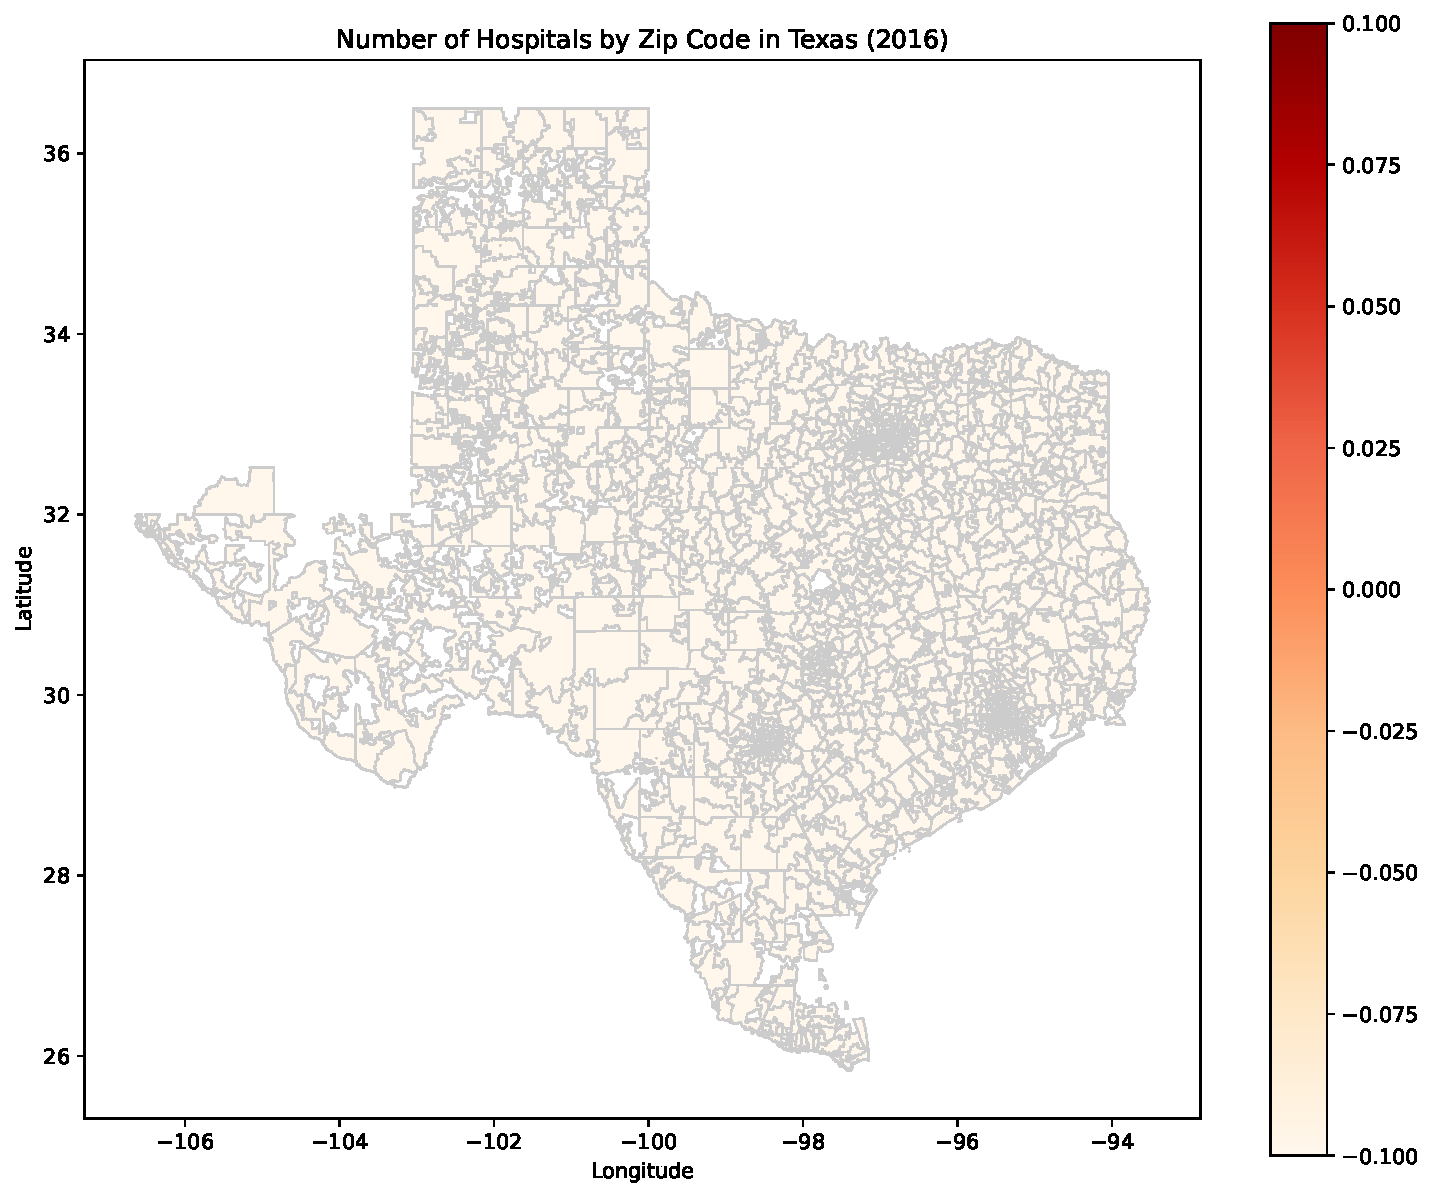
\includegraphics[keepaspectratio]{pset4_template_files/figure-pdf/cell-13-output-2.pdf}}

\subsection{Calculate zip code's distance to the nearest hospital (20
pts)
(*)}\label{calculate-zip-codes-distance-to-the-nearest-hospital-20-pts}

\begin{enumerate}
\def\labelenumi{\arabic{enumi}.}
\tightlist
\item
\end{enumerate}

\begin{Shaded}
\begin{Highlighting}[]
\CommentTok{\# import sys}
\CommentTok{\# sys.setrecursionlimit(200000) }

\ImportTok{import}\NormalTok{ geopandas }\ImportTok{as}\NormalTok{ gpd}
\NormalTok{shapefile\_path }\OperatorTok{=} \StringTok{\textquotesingle{}gz\_2010\_us\_860\_00\_500k/gz\_2010\_us\_860\_00\_500k.shp\textquotesingle{}}
\NormalTok{zips\_all }\OperatorTok{=}\NormalTok{ gpd.read\_file(shapefile\_path)}
\end{Highlighting}
\end{Shaded}

\begin{Shaded}
\begin{Highlighting}[]
\NormalTok{zips\_all\_centroids }\OperatorTok{=}\NormalTok{ zips\_all.copy()}
\NormalTok{zips\_all\_centroids[}\StringTok{\textquotesingle{}centroid\textquotesingle{}}\NormalTok{] }\OperatorTok{=}\NormalTok{ zips\_all.geometry.centroid}
\NormalTok{zips\_all\_centroids }\OperatorTok{=}\NormalTok{ zips\_all\_centroids.set\_geometry(}\StringTok{\textquotesingle{}centroid\textquotesingle{}}\NormalTok{)}
\end{Highlighting}
\end{Shaded}

\begin{Shaded}
\begin{Highlighting}[]
\BuiltInTok{print}\NormalTok{(}\StringTok{"Dimensions of the GeoDataFrame:"}\NormalTok{, zips\_all\_centroids.shape)}
\end{Highlighting}
\end{Shaded}

\begin{verbatim}
Dimensions of the GeoDataFrame: (33120, 7)
\end{verbatim}

GEO\_ID: A unique identifier for each area, formatted with a prefix
(8600000US) plus the ZIP code. ZCTA5: The 5-digit ZIP Code Tabulation
Area (ZCTA), a Census Bureau representation of a ZIP code area. NAME:
The ZIP code associated with each ZCTA. LSAD: Indicates that each row is
a 5-digit ZCTA. CENSUSAREA: The land area of the ZCTA in square miles.
geometry: The shape of each ZCTA, as either: POLYGON: A single shape.
MULTIPOLYGON: Multiple shapes, used if a ZIP code area is split into
separate parts. 2.

\begin{Shaded}
\begin{Highlighting}[]
\NormalTok{texas\_zip\_prefixes }\OperatorTok{=}\NormalTok{ [}\StringTok{\textquotesingle{}75\textquotesingle{}}\NormalTok{, }\StringTok{\textquotesingle{}76\textquotesingle{}}\NormalTok{, }\StringTok{\textquotesingle{}77\textquotesingle{}}\NormalTok{, }\StringTok{\textquotesingle{}78\textquotesingle{}}\NormalTok{, }\StringTok{\textquotesingle{}79\textquotesingle{}}\NormalTok{]  }\CommentTok{\# Texas ZIP code prefixes}
\NormalTok{zips\_texas\_centroids }\OperatorTok{=}\NormalTok{ zips\_all\_centroids[zips\_all\_centroids[}\StringTok{\textquotesingle{}ZCTA5\textquotesingle{}}\NormalTok{].}\BuiltInTok{str}\NormalTok{.startswith(}\BuiltInTok{tuple}\NormalTok{(texas\_zip\_prefixes))]}
\NormalTok{unique\_texas\_zips }\OperatorTok{=}\NormalTok{ zips\_texas\_centroids[}\StringTok{\textquotesingle{}ZCTA5\textquotesingle{}}\NormalTok{].nunique()}
\end{Highlighting}
\end{Shaded}

\begin{Shaded}
\begin{Highlighting}[]
\ImportTok{from}\NormalTok{ shapely.ops }\ImportTok{import}\NormalTok{ unary\_union}

\NormalTok{texas\_polygon }\OperatorTok{=}\NormalTok{ unary\_union(zips\_texas\_centroids.geometry).convex\_hull}
\CommentTok{\# making this multipolygon into a big polygon with convex\_hull}
\KeywordTok{def}\NormalTok{ polygons\_intersect\_or\_touch(polygon1, polygon2):}
    \ControlFlowTok{return}\NormalTok{ polygon1.intersects(polygon2) }\KeywordTok{or}\NormalTok{ polygon1.touches(polygon2)}
\end{Highlighting}
\end{Shaded}

\begin{Shaded}
\begin{Highlighting}[]
\NormalTok{zips\_texas\_borderstates\_centroids }\OperatorTok{=}\NormalTok{ zips\_all\_centroids[zips\_all\_centroids.geometry.}\BuiltInTok{apply}\NormalTok{(}\KeywordTok{lambda}\NormalTok{ x: polygons\_intersect\_or\_touch(texas\_polygon, x))]}

\NormalTok{unique\_texas\_border\_zips }\OperatorTok{=}\NormalTok{ zips\_texas\_borderstates\_centroids[}\StringTok{\textquotesingle{}ZCTA5\textquotesingle{}}\NormalTok{].nunique()}
\BuiltInTok{print}\NormalTok{(}\StringTok{"Number of unique ZIP codes in Texas:"}\NormalTok{, unique\_texas\_zips)}
\BuiltInTok{print}\NormalTok{(}\StringTok{"Number of unique ZIP codes in Texas and border states:"}\NormalTok{, unique\_texas\_border\_zips)}
\end{Highlighting}
\end{Shaded}

\begin{verbatim}
Number of unique ZIP codes in Texas: 1935
Number of unique ZIP codes in Texas and border states: 2179
\end{verbatim}

\begin{enumerate}
\def\labelenumi{\arabic{enumi}.}
\setcounter{enumi}{2}
\tightlist
\item
\end{enumerate}

\begin{Shaded}
\begin{Highlighting}[]
\NormalTok{zips\_texas\_borderstates\_centroids[}\StringTok{\textquotesingle{}ZCTA5\textquotesingle{}}\NormalTok{] }\OperatorTok{=}\NormalTok{ pd.to\_numeric(zips\_texas\_borderstates\_centroids[}\StringTok{\textquotesingle{}ZCTA5\textquotesingle{}}\NormalTok{], errors}\OperatorTok{=}\StringTok{\textquotesingle{}coerce\textquotesingle{}}\NormalTok{)}
\NormalTok{pos2016[}\StringTok{\textquotesingle{}ZIP\_CD\textquotesingle{}}\NormalTok{] }\OperatorTok{=}\NormalTok{ pd.to\_numeric(pos2016[}\StringTok{\textquotesingle{}ZIP\_CD\textquotesingle{}}\NormalTok{], errors}\OperatorTok{=}\StringTok{\textquotesingle{}coerce\textquotesingle{}}\NormalTok{)}


\NormalTok{hospital\_zip\_codes\_2016 }\OperatorTok{=}\NormalTok{ pos2016[[}\StringTok{\textquotesingle{}ZIP\_CD\textquotesingle{}}\NormalTok{]].drop\_duplicates()}
\NormalTok{zips\_withhospital\_centroids }\OperatorTok{=}\NormalTok{ zips\_texas\_borderstates\_centroids.merge(}
\NormalTok{    hospital\_zip\_codes\_2016,}
\NormalTok{    how}\OperatorTok{=}\StringTok{\textquotesingle{}inner\textquotesingle{}}\NormalTok{,}
\NormalTok{    left\_on}\OperatorTok{=}\StringTok{\textquotesingle{}ZCTA5\textquotesingle{}}\NormalTok{,}
\NormalTok{    right\_on}\OperatorTok{=}\StringTok{\textquotesingle{}ZIP\_CD\textquotesingle{}}
\NormalTok{)}
\NormalTok{unique\_hospital\_zips }\OperatorTok{=}\NormalTok{ zips\_withhospital\_centroids[}\StringTok{\textquotesingle{}ZCTA5\textquotesingle{}}\NormalTok{].nunique()}
\BuiltInTok{print}\NormalTok{(}\StringTok{"Number of unique ZIP codes in Texas and bordering states with at least one hospital in 2016:"}\NormalTok{, unique\_hospital\_zips)}
\end{Highlighting}
\end{Shaded}

\begin{verbatim}
Number of unique ZIP codes in Texas and bordering states with at least one hospital in 2016: 1292
\end{verbatim}

Number of unique ZIP codes in Texas and bordering states with at least
one hospital in 2016: 1292.

The merge function joins zips\_texas\_borderstates\_centroids and
hospital\_zip\_codes\_2016:

how=`inner': An inner join keeps only the rows where ZCTA5 in
zips\_texas\_borderstates\_centroids matches ZIP\_CD in
hospital\_zip\_codes\_2016.

left\_on=`ZCTA5', right\_on=`ZIP\_CD': Specifies the columns to match
on. 4.

\begin{Shaded}
\begin{Highlighting}[]
\ImportTok{import}\NormalTok{ time}
\ImportTok{from}\NormalTok{ shapely.ops }\ImportTok{import}\NormalTok{ nearest\_points}

\NormalTok{subset\_zips\_texas\_centroids }\OperatorTok{=}\NormalTok{ zips\_texas\_centroids.head(}\DecValTok{10}\NormalTok{)}
\KeywordTok{def}\NormalTok{ calculate\_nearest\_distance(row, target\_gdf):}
\NormalTok{    nearest\_geom }\OperatorTok{=}\NormalTok{ nearest\_points(row.geometry, target\_gdf.unary\_union)[}\DecValTok{1}\NormalTok{]}
    \ControlFlowTok{return}\NormalTok{ row.geometry.distance(nearest\_geom)}

\NormalTok{start\_time }\OperatorTok{=}\NormalTok{ time.time()}
\NormalTok{subset\_zips\_texas\_centroids[}\StringTok{\textquotesingle{}nearest\_distance\textquotesingle{}}\NormalTok{] }\OperatorTok{=}\NormalTok{ subset\_zips\_texas\_centroids.}\BuiltInTok{apply}\NormalTok{(}
\NormalTok{    calculate\_nearest\_distance, target\_gdf}\OperatorTok{=}\NormalTok{zips\_withhospital\_centroids, axis}\OperatorTok{=}\DecValTok{1}
\NormalTok{)}

\NormalTok{elapsed\_time }\OperatorTok{=}\NormalTok{ time.time() }\OperatorTok{{-}}\NormalTok{ start\_time}
\BuiltInTok{print}\NormalTok{(}\SpecialStringTok{f"Time taken for 10 ZIP codes: }\SpecialCharTok{\{}\NormalTok{elapsed\_time}\SpecialCharTok{:.2f\}}\SpecialStringTok{ seconds"}\NormalTok{)}
\end{Highlighting}
\end{Shaded}

\begin{verbatim}
Time taken for 10 ZIP codes: 0.03 seconds
\end{verbatim}

\begin{Shaded}
\begin{Highlighting}[]
\NormalTok{total\_rows }\OperatorTok{=} \BuiltInTok{len}\NormalTok{(zips\_texas\_centroids)}
\NormalTok{estimated\_time }\OperatorTok{=}\NormalTok{ (elapsed\_time }\OperatorTok{/} \DecValTok{10}\NormalTok{) }\OperatorTok{*}\NormalTok{ total\_rows}
\BuiltInTok{print}\NormalTok{(}\SpecialStringTok{f"Estimated time for full dataset: }\SpecialCharTok{\{}\NormalTok{estimated\_time }\OperatorTok{/} \DecValTok{60}\SpecialCharTok{:.2f\}}\SpecialStringTok{ minutes"}\NormalTok{)}
\end{Highlighting}
\end{Shaded}

\begin{verbatim}
Estimated time for full dataset: 0.10 minutes
\end{verbatim}

\begin{verbatim}
a.
\end{verbatim}

\begin{Shaded}
\begin{Highlighting}[]
\NormalTok{start\_time }\OperatorTok{=}\NormalTok{ time.time()}

\NormalTok{zips\_texas\_centroids[}\StringTok{\textquotesingle{}nearest\_distance\textquotesingle{}}\NormalTok{] }\OperatorTok{=}\NormalTok{ zips\_texas\_centroids.}\BuiltInTok{apply}\NormalTok{(}
\NormalTok{calculate\_nearest\_distance, target\_gdf}\OperatorTok{=}\NormalTok{zips\_withhospital\_centroids, axis}\OperatorTok{=}\DecValTok{1}
\NormalTok{)}

\NormalTok{full\_elapsed\_time }\OperatorTok{=}\NormalTok{ time.time() }\OperatorTok{{-}}\NormalTok{ start\_time}
\BuiltInTok{print}\NormalTok{(}\SpecialStringTok{f"Time taken for full dataset: }\SpecialCharTok{\{}\NormalTok{full\_elapsed\_time }\OperatorTok{/} \DecValTok{60}\SpecialCharTok{:.2f\}}\SpecialStringTok{ minutes"}\NormalTok{)}
\end{Highlighting}
\end{Shaded}

\begin{verbatim}
Time taken for full dataset: 0.09 minutes
\end{verbatim}

Estimated time for full dataset: 0.14 minutes Time taken for full
dataset: 0.08 minutes They were quite off. b. The .prj file indicates
that the coordinate system is GCS\_North\_American\_1983, with units in
degrees.

\begin{Shaded}
\begin{Highlighting}[]
\NormalTok{zips\_texas\_centroids }\OperatorTok{=}\NormalTok{ zips\_texas\_centroids.to\_crs(}\StringTok{"EPSG:5070"}\NormalTok{)}
\NormalTok{zips\_withhospital\_centroids }\OperatorTok{=}\NormalTok{ zips\_withhospital\_centroids.to\_crs(}\StringTok{"EPSG:5070"}\NormalTok{)}
\NormalTok{zips\_texas\_centroids[}\StringTok{\textquotesingle{}nearest\_distance\_meters\textquotesingle{}}\NormalTok{] }\OperatorTok{=}\NormalTok{ zips\_texas\_centroids.}\BuiltInTok{apply}\NormalTok{(}
\NormalTok{    calculate\_nearest\_distance, target\_gdf}\OperatorTok{=}\NormalTok{zips\_withhospital\_centroids, axis}\OperatorTok{=}\DecValTok{1}
\NormalTok{)}
\NormalTok{conversion\_factor }\OperatorTok{=} \FloatTok{0.000621371}  \CommentTok{\# 1 meter ≈ 0.000621371 miles}
\NormalTok{zips\_texas\_centroids[}\StringTok{\textquotesingle{}nearest\_distance\_miles\textquotesingle{}}\NormalTok{] }\OperatorTok{=}\NormalTok{ zips\_texas\_centroids[}\StringTok{\textquotesingle{}nearest\_distance\_meters\textquotesingle{}}\NormalTok{] }\OperatorTok{*}\NormalTok{ conversion\_factor}

\NormalTok{average\_distance\_miles }\OperatorTok{=}\NormalTok{ zips\_texas\_centroids[}\StringTok{\textquotesingle{}nearest\_distance\_miles\textquotesingle{}}\NormalTok{].mean()}
\end{Highlighting}
\end{Shaded}

\begin{enumerate}
\def\labelenumi{\arabic{enumi}.}
\setcounter{enumi}{4}
\tightlist
\item
  \begin{enumerate}
  \def\labelenumii{\alph{enumii}.}
  \tightlist
  \item
    In miles.
  \item
  \end{enumerate}
\end{enumerate}

\begin{Shaded}
\begin{Highlighting}[]
\BuiltInTok{print}\NormalTok{(}\SpecialStringTok{f"Average distance to the nearest hospital for each ZIP code in Texas (in miles): }\SpecialCharTok{\{}\NormalTok{average\_distance\_miles}\SpecialCharTok{:.2f\}}\SpecialStringTok{"}\NormalTok{)}
\end{Highlighting}
\end{Shaded}

\begin{verbatim}
Average distance to the nearest hospital for each ZIP code in Texas (in miles): 217.29
\end{verbatim}

\begin{verbatim}
c.
\end{verbatim}

\begin{Shaded}
\begin{Highlighting}[]
\ImportTok{import}\NormalTok{ matplotlib.pyplot }\ImportTok{as}\NormalTok{ plt}

\NormalTok{fig, ax }\OperatorTok{=}\NormalTok{ plt.subplots(}\DecValTok{1}\NormalTok{, }\DecValTok{1}\NormalTok{, figsize}\OperatorTok{=}\NormalTok{(}\DecValTok{10}\NormalTok{, }\DecValTok{10}\NormalTok{))}
\NormalTok{zips\_texas\_centroids.plot(column}\OperatorTok{=}\StringTok{\textquotesingle{}nearest\_distance\_miles\textquotesingle{}}\NormalTok{, cmap}\OperatorTok{=}\StringTok{\textquotesingle{}coolwarm\textquotesingle{}}\NormalTok{, linewidth}\OperatorTok{=}\FloatTok{0.8}\NormalTok{, ax}\OperatorTok{=}\NormalTok{ax, edgecolor}\OperatorTok{=}\StringTok{\textquotesingle{}0.8\textquotesingle{}}\NormalTok{, legend}\OperatorTok{=}\VariableTok{True}\NormalTok{)}

\NormalTok{ax.set\_title(}\StringTok{"Distance to Nearest Hospital for Each ZIP Code in Texas (in miles)"}\NormalTok{)}
\NormalTok{ax.set\_axis\_off()}
\NormalTok{plt.show()}
\end{Highlighting}
\end{Shaded}

\pandocbounded{\includegraphics[keepaspectratio]{pset4_template_files/figure-pdf/cell-26-output-1.pdf}}

This makes sense, as ZIP codes closer to the U.S. border tend to have
greater distances to the nearest hospital compared to those located
further inland.

\subsection{Effects of closures on access in Texas (15
pts)}\label{effects-of-closures-on-access-in-texas-15-pts}

\begin{enumerate}
\def\labelenumi{\arabic{enumi}.}
\tightlist
\item
\end{enumerate}

\begin{Shaded}
\begin{Highlighting}[]
\NormalTok{texas\_zip\_prefixes }\OperatorTok{=}\NormalTok{ [}\StringTok{\textquotesingle{}75\textquotesingle{}}\NormalTok{, }\StringTok{\textquotesingle{}76\textquotesingle{}}\NormalTok{, }\StringTok{\textquotesingle{}77\textquotesingle{}}\NormalTok{, }\StringTok{\textquotesingle{}78\textquotesingle{}}\NormalTok{, }\StringTok{\textquotesingle{}79\textquotesingle{}}\NormalTok{]}
\NormalTok{corrected\_closures[}\StringTok{\textquotesingle{}ZIP\_CD\textquotesingle{}}\NormalTok{] }\OperatorTok{=}\NormalTok{ corrected\_closures[}\StringTok{\textquotesingle{}ZIP\_CD\textquotesingle{}}\NormalTok{].astype(}\BuiltInTok{str}\NormalTok{)}

\NormalTok{texas\_closures }\OperatorTok{=}\NormalTok{ corrected\_closures[corrected\_closures[}\StringTok{\textquotesingle{}ZIP\_CD\textquotesingle{}}\NormalTok{].}\BuiltInTok{str}\NormalTok{.startswith(}\BuiltInTok{tuple}\NormalTok{(texas\_zip\_prefixes))]}

\NormalTok{closure\_counts }\OperatorTok{=}\NormalTok{ texas\_closures.groupby(}\StringTok{\textquotesingle{}ZIP\_CD\textquotesingle{}}\NormalTok{).size().reset\_index(name}\OperatorTok{=}\StringTok{\textquotesingle{}closure\_count\textquotesingle{}}\NormalTok{)}

\NormalTok{closure\_counts\_sorted }\OperatorTok{=}\NormalTok{ closure\_counts.sort\_values(by}\OperatorTok{=}\StringTok{\textquotesingle{}closure\_count\textquotesingle{}}\NormalTok{, ascending}\OperatorTok{=}\VariableTok{False}\NormalTok{)}

\BuiltInTok{print}\NormalTok{(}\StringTok{"Texas Zip Codes and the Number of Hospital Closures (2016{-}2019):"}\NormalTok{)}
\BuiltInTok{print}\NormalTok{(closure\_counts\_sorted)}
\end{Highlighting}
\end{Shaded}

\begin{verbatim}
Texas Zip Codes and the Number of Hospital Closures (2016-2019):
      ZIP_CD  closure_count
177  77036.0             55
233  77477.0             32
193  77074.0             26
323  78501.0             14
38   75150.0             13
..       ...            ...
198  77082.0              1
201  77089.0              1
202  77090.0              1
1    75010.0              1
406  79938.0              1

[407 rows x 2 columns]
\end{verbatim}

\begin{enumerate}
\def\labelenumi{\arabic{enumi}.}
\setcounter{enumi}{1}
\tightlist
\item
\end{enumerate}

\begin{Shaded}
\begin{Highlighting}[]
\ImportTok{import}\NormalTok{ os}
\ImportTok{import}\NormalTok{ geopandas }\ImportTok{as}\NormalTok{ gpd}
\ImportTok{import}\NormalTok{ pandas }\ImportTok{as}\NormalTok{ pd}
\ImportTok{import}\NormalTok{ matplotlib.pyplot }\ImportTok{as}\NormalTok{ plt}
\NormalTok{os.environ[}\StringTok{"PROJ\_LIB"}\NormalTok{] }\OperatorTok{=} \StringTok{"/opt/homebrew/Cellar/proj/9.5.0/share/proj"}

\NormalTok{texas\_zip\_prefixes }\OperatorTok{=}\NormalTok{ [}\StringTok{\textquotesingle{}75\textquotesingle{}}\NormalTok{, }\StringTok{\textquotesingle{}76\textquotesingle{}}\NormalTok{, }\StringTok{\textquotesingle{}77\textquotesingle{}}\NormalTok{, }\StringTok{\textquotesingle{}78\textquotesingle{}}\NormalTok{, }\StringTok{\textquotesingle{}79\textquotesingle{}}\NormalTok{]}
\NormalTok{corrected\_closures[}\StringTok{\textquotesingle{}ZIP\_CD\textquotesingle{}}\NormalTok{] }\OperatorTok{=}\NormalTok{ corrected\_closures[}\StringTok{\textquotesingle{}ZIP\_CD\textquotesingle{}}\NormalTok{].astype(}\BuiltInTok{str}\NormalTok{).}\BuiltInTok{str}\NormalTok{.split(}\StringTok{\textquotesingle{}.\textquotesingle{}}\NormalTok{).}\BuiltInTok{str}\NormalTok{[}\DecValTok{0}\NormalTok{].}\BuiltInTok{str}\NormalTok{.zfill(}\DecValTok{5}\NormalTok{)}
\NormalTok{corrected\_closures\_texas }\OperatorTok{=}\NormalTok{ corrected\_closures[corrected\_closures[}\StringTok{\textquotesingle{}ZIP\_CD\textquotesingle{}}\NormalTok{].}\BuiltInTok{str}\NormalTok{[:}\DecValTok{2}\NormalTok{].isin(texas\_zip\_prefixes)]}

\NormalTok{closure\_counts }\OperatorTok{=}\NormalTok{ corrected\_closures\_texas.groupby(}\StringTok{\textquotesingle{}ZIP\_CD\textquotesingle{}}\NormalTok{).size().reset\_index(name}\OperatorTok{=}\StringTok{\textquotesingle{}closure\_count\textquotesingle{}}\NormalTok{)}

\NormalTok{shapefile\_path }\OperatorTok{=} \StringTok{"gz\_2010\_us\_860\_00\_500k/gz\_2010\_us\_860\_00\_500k.shp"}
\NormalTok{zipcodes }\OperatorTok{=}\NormalTok{ gpd.read\_file(shapefile\_path)}
\NormalTok{zipcodes[}\StringTok{\textquotesingle{}ZCTA5\textquotesingle{}}\NormalTok{] }\OperatorTok{=}\NormalTok{ zipcodes[}\StringTok{\textquotesingle{}ZCTA5\textquotesingle{}}\NormalTok{].astype(}\BuiltInTok{str}\NormalTok{).}\BuiltInTok{str}\NormalTok{.zfill(}\DecValTok{5}\NormalTok{)}
\NormalTok{texas\_zipcodes }\OperatorTok{=}\NormalTok{ zipcodes[zipcodes[}\StringTok{\textquotesingle{}ZCTA5\textquotesingle{}}\NormalTok{].}\BuiltInTok{str}\NormalTok{[:}\DecValTok{2}\NormalTok{].isin(texas\_zip\_prefixes)]}

\NormalTok{texas\_zipcodes }\OperatorTok{=}\NormalTok{ texas\_zipcodes.merge(closure\_counts, left\_on}\OperatorTok{=}\StringTok{\textquotesingle{}ZCTA5\textquotesingle{}}\NormalTok{, right\_on}\OperatorTok{=}\StringTok{\textquotesingle{}ZIP\_CD\textquotesingle{}}\NormalTok{, how}\OperatorTok{=}\StringTok{\textquotesingle{}left\textquotesingle{}}\NormalTok{)}
\NormalTok{texas\_zipcodes[}\StringTok{\textquotesingle{}closure\_count\textquotesingle{}}\NormalTok{] }\OperatorTok{=}\NormalTok{ texas\_zipcodes[}\StringTok{\textquotesingle{}closure\_count\textquotesingle{}}\NormalTok{].fillna(}\DecValTok{0}\NormalTok{)}

\NormalTok{fig, ax }\OperatorTok{=}\NormalTok{ plt.subplots(}\DecValTok{1}\NormalTok{, }\DecValTok{1}\NormalTok{, figsize}\OperatorTok{=}\NormalTok{(}\DecValTok{12}\NormalTok{, }\DecValTok{10}\NormalTok{))}
\NormalTok{texas\_zipcodes.plot(column}\OperatorTok{=}\StringTok{\textquotesingle{}closure\_count\textquotesingle{}}\NormalTok{, cmap}\OperatorTok{=}\StringTok{\textquotesingle{}OrRd\textquotesingle{}}\NormalTok{, linewidth}\OperatorTok{=}\FloatTok{0.8}\NormalTok{, ax}\OperatorTok{=}\NormalTok{ax, edgecolor}\OperatorTok{=}\StringTok{\textquotesingle{}0.8\textquotesingle{}}\NormalTok{, legend}\OperatorTok{=}\VariableTok{True}\NormalTok{)}
\NormalTok{plt.title(}\StringTok{\textquotesingle{}Directly Affected Texas ZIP Codes by Hospital Closures (2016{-}2019)\textquotesingle{}}\NormalTok{)}
\NormalTok{plt.xlabel(}\StringTok{\textquotesingle{}Longitude\textquotesingle{}}\NormalTok{)}
\NormalTok{plt.ylabel(}\StringTok{\textquotesingle{}Latitude\textquotesingle{}}\NormalTok{)}
\NormalTok{plt.show()}

\NormalTok{directly\_affected\_zipcodes }\OperatorTok{=}\NormalTok{ texas\_zipcodes[texas\_zipcodes[}\StringTok{\textquotesingle{}closure\_count\textquotesingle{}}\NormalTok{] }\OperatorTok{\textgreater{}} \DecValTok{0}\NormalTok{]}
\BuiltInTok{print}\NormalTok{(}\StringTok{"Number of directly affected Texas ZIP codes:"}\NormalTok{, directly\_affected\_zipcodes.shape[}\DecValTok{0}\NormalTok{])}
\end{Highlighting}
\end{Shaded}

\pandocbounded{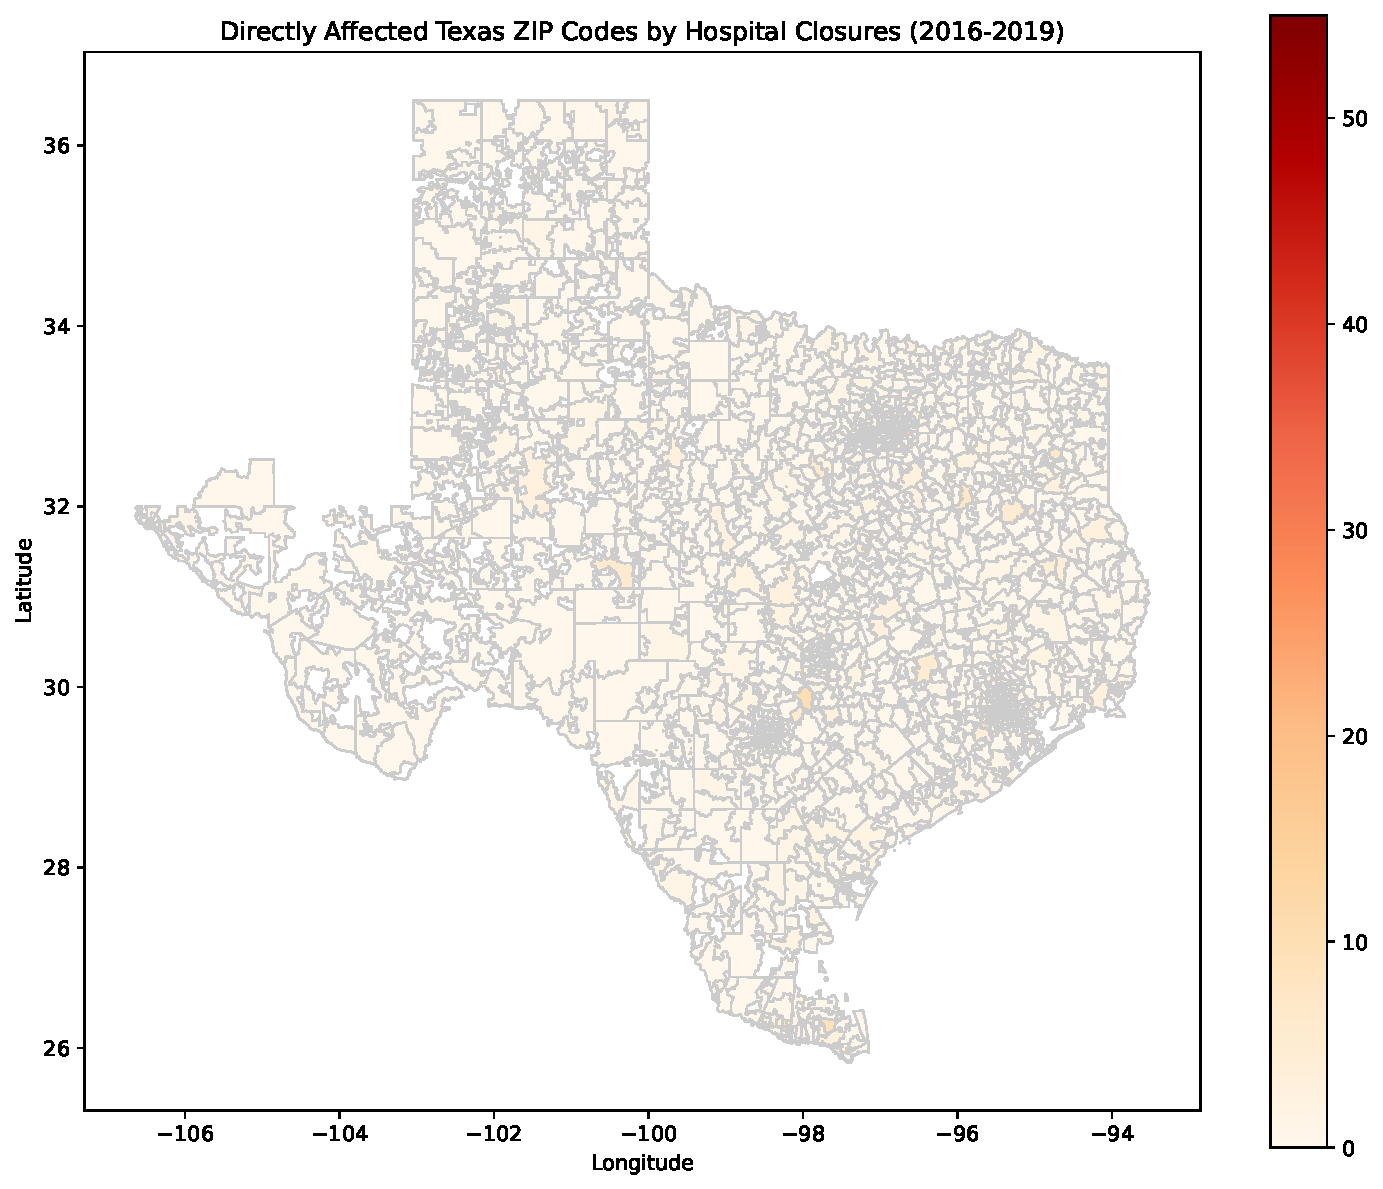
\includegraphics[keepaspectratio]{pset4_template_files/figure-pdf/cell-28-output-1.pdf}}

\begin{verbatim}
Number of directly affected Texas ZIP codes: 383
\end{verbatim}

\begin{enumerate}
\def\labelenumi{\arabic{enumi}.}
\setcounter{enumi}{2}
\tightlist
\item
\end{enumerate}

\begin{Shaded}
\begin{Highlighting}[]
\ImportTok{import}\NormalTok{ geopandas }\ImportTok{as}\NormalTok{ gpd}
\ImportTok{from}\NormalTok{ geopandas.tools }\ImportTok{import}\NormalTok{ sjoin}
\ImportTok{import}\NormalTok{ pandas }\ImportTok{as}\NormalTok{ pd}
\ImportTok{import}\NormalTok{ matplotlib.pyplot }\ImportTok{as}\NormalTok{ plt}

\NormalTok{directly\_affected\_zipcodes\_gdf }\OperatorTok{=}\NormalTok{ texas\_zipcodes[texas\_zipcodes[}\StringTok{\textquotesingle{}closure\_count\textquotesingle{}}\NormalTok{] }\OperatorTok{\textgreater{}} \DecValTok{0}\NormalTok{]}

\NormalTok{directly\_affected\_zipcodes\_gdf }\OperatorTok{=}\NormalTok{ gpd.GeoDataFrame(directly\_affected\_zipcodes\_gdf, geometry}\OperatorTok{=}\StringTok{\textquotesingle{}geometry\textquotesingle{}}\NormalTok{, crs}\OperatorTok{=}\StringTok{"EPSG:4326"}\NormalTok{)}

\NormalTok{directly\_affected\_zipcodes\_gdf }\OperatorTok{=}\NormalTok{ directly\_affected\_zipcodes\_gdf.to\_crs(epsg}\OperatorTok{=}\DecValTok{2163}\NormalTok{) }

\NormalTok{buffered\_zones }\OperatorTok{=}\NormalTok{ directly\_affected\_zipcodes\_gdf.copy()}
\NormalTok{buffered\_zones[}\StringTok{\textquotesingle{}geometry\textquotesingle{}}\NormalTok{] }\OperatorTok{=}\NormalTok{ directly\_affected\_zipcodes\_gdf.geometry.}\BuiltInTok{buffer}\NormalTok{(}\DecValTok{16093}\NormalTok{)  }\CommentTok{\# 10 miles in meters}

\NormalTok{texas\_zipcodes\_projected }\OperatorTok{=}\NormalTok{ texas\_zipcodes.to\_crs(epsg}\OperatorTok{=}\DecValTok{2163}\NormalTok{)}

\NormalTok{indirectly\_affected\_zipcodes }\OperatorTok{=}\NormalTok{ sjoin(texas\_zipcodes\_projected, buffered\_zones, how}\OperatorTok{=}\StringTok{"inner"}\NormalTok{, predicate}\OperatorTok{=}\StringTok{"intersects"}\NormalTok{)}

\BuiltInTok{print}\NormalTok{(}\StringTok{"Columns in indirectly\_affected\_zipcodes after spatial join:"}\NormalTok{, indirectly\_affected\_zipcodes.columns)}

\ControlFlowTok{if} \StringTok{\textquotesingle{}ZCTA5\textquotesingle{}} \KeywordTok{in}\NormalTok{ indirectly\_affected\_zipcodes.columns:}
\NormalTok{    column\_name }\OperatorTok{=} \StringTok{\textquotesingle{}ZCTA5\textquotesingle{}}
\ControlFlowTok{else}\NormalTok{:}
\NormalTok{    column\_name }\OperatorTok{=}\NormalTok{ indirectly\_affected\_zipcodes.columns[}\DecValTok{0}\NormalTok{]}


\NormalTok{indirectly\_affected\_zipcodes }\OperatorTok{=}\NormalTok{ indirectly\_affected\_zipcodes[}
    \OperatorTok{\textasciitilde{}}\NormalTok{indirectly\_affected\_zipcodes[column\_name].isin(directly\_affected\_zipcodes\_gdf[}\StringTok{\textquotesingle{}ZCTA5\textquotesingle{}}\NormalTok{])}
\NormalTok{]}

\NormalTok{num\_indirectly\_affected }\OperatorTok{=}\NormalTok{ indirectly\_affected\_zipcodes[column\_name].nunique()}
\BuiltInTok{print}\NormalTok{(}\StringTok{"Number of indirectly affected Texas ZIP codes:"}\NormalTok{, num\_indirectly\_affected)}
\end{Highlighting}
\end{Shaded}

\begin{verbatim}
Columns in indirectly_affected_zipcodes after spatial join: Index(['GEO_ID_left', 'ZCTA5_left', 'NAME_left', 'LSAD_left',
       'CENSUSAREA_left', 'geometry', 'ZIP_CD_left', 'closure_count_left',
       'index_right', 'GEO_ID_right', 'ZCTA5_right', 'NAME_right',
       'LSAD_right', 'CENSUSAREA_right', 'ZIP_CD_right',
       'closure_count_right'],
      dtype='object')
Number of indirectly affected Texas ZIP codes: 1705
\end{verbatim}

\begin{enumerate}
\def\labelenumi{\arabic{enumi}.}
\setcounter{enumi}{3}
\tightlist
\item
\end{enumerate}

\begin{Shaded}
\begin{Highlighting}[]
\ImportTok{import}\NormalTok{ geopandas }\ImportTok{as}\NormalTok{ gpd}
\ImportTok{import}\NormalTok{ matplotlib.pyplot }\ImportTok{as}\NormalTok{ plt}

\NormalTok{texas\_zipcodes[}\StringTok{\textquotesingle{}impact\_status\textquotesingle{}}\NormalTok{] }\OperatorTok{=} \StringTok{\textquotesingle{}Unaffected\textquotesingle{}}  \CommentTok{\# Default to unaffected}
\NormalTok{texas\_zipcodes.loc[texas\_zipcodes[}\StringTok{\textquotesingle{}ZCTA5\textquotesingle{}}\NormalTok{].isin(directly\_affected\_zipcodes\_gdf[}\StringTok{\textquotesingle{}ZCTA5\textquotesingle{}}\NormalTok{]), }\StringTok{\textquotesingle{}impact\_status\textquotesingle{}}\NormalTok{] }\OperatorTok{=} \StringTok{\textquotesingle{}Directly Affected\textquotesingle{}}

\NormalTok{texas\_zipcodes.loc[texas\_zipcodes[}\StringTok{\textquotesingle{}ZCTA5\textquotesingle{}}\NormalTok{].isin(indirectly\_affected\_zipcodes[column\_name]), }\StringTok{\textquotesingle{}impact\_status\textquotesingle{}}\NormalTok{] }\OperatorTok{=} \StringTok{\textquotesingle{}Indirectly Affected\textquotesingle{}}

\NormalTok{fig, ax }\OperatorTok{=}\NormalTok{ plt.subplots(}\DecValTok{1}\NormalTok{, }\DecValTok{1}\NormalTok{, figsize}\OperatorTok{=}\NormalTok{(}\DecValTok{12}\NormalTok{, }\DecValTok{10}\NormalTok{))}
\NormalTok{texas\_zipcodes.plot(column}\OperatorTok{=}\StringTok{\textquotesingle{}impact\_status\textquotesingle{}}\NormalTok{, cmap}\OperatorTok{=}\StringTok{\textquotesingle{}coolwarm\textquotesingle{}}\NormalTok{, linewidth}\OperatorTok{=}\FloatTok{0.8}\NormalTok{, ax}\OperatorTok{=}\NormalTok{ax, edgecolor}\OperatorTok{=}\StringTok{\textquotesingle{}0.8\textquotesingle{}}\NormalTok{, legend}\OperatorTok{=}\VariableTok{True}\NormalTok{)}

\NormalTok{plt.title(}\StringTok{\textquotesingle{}Texas ZIP Codes Affected by Hospital Closures (2016{-}2019)\textquotesingle{}}\NormalTok{)}
\NormalTok{plt.xlabel(}\StringTok{\textquotesingle{}Longitude\textquotesingle{}}\NormalTok{)}
\NormalTok{plt.ylabel(}\StringTok{\textquotesingle{}Latitude\textquotesingle{}}\NormalTok{)}
\NormalTok{plt.show()}
\end{Highlighting}
\end{Shaded}

\pandocbounded{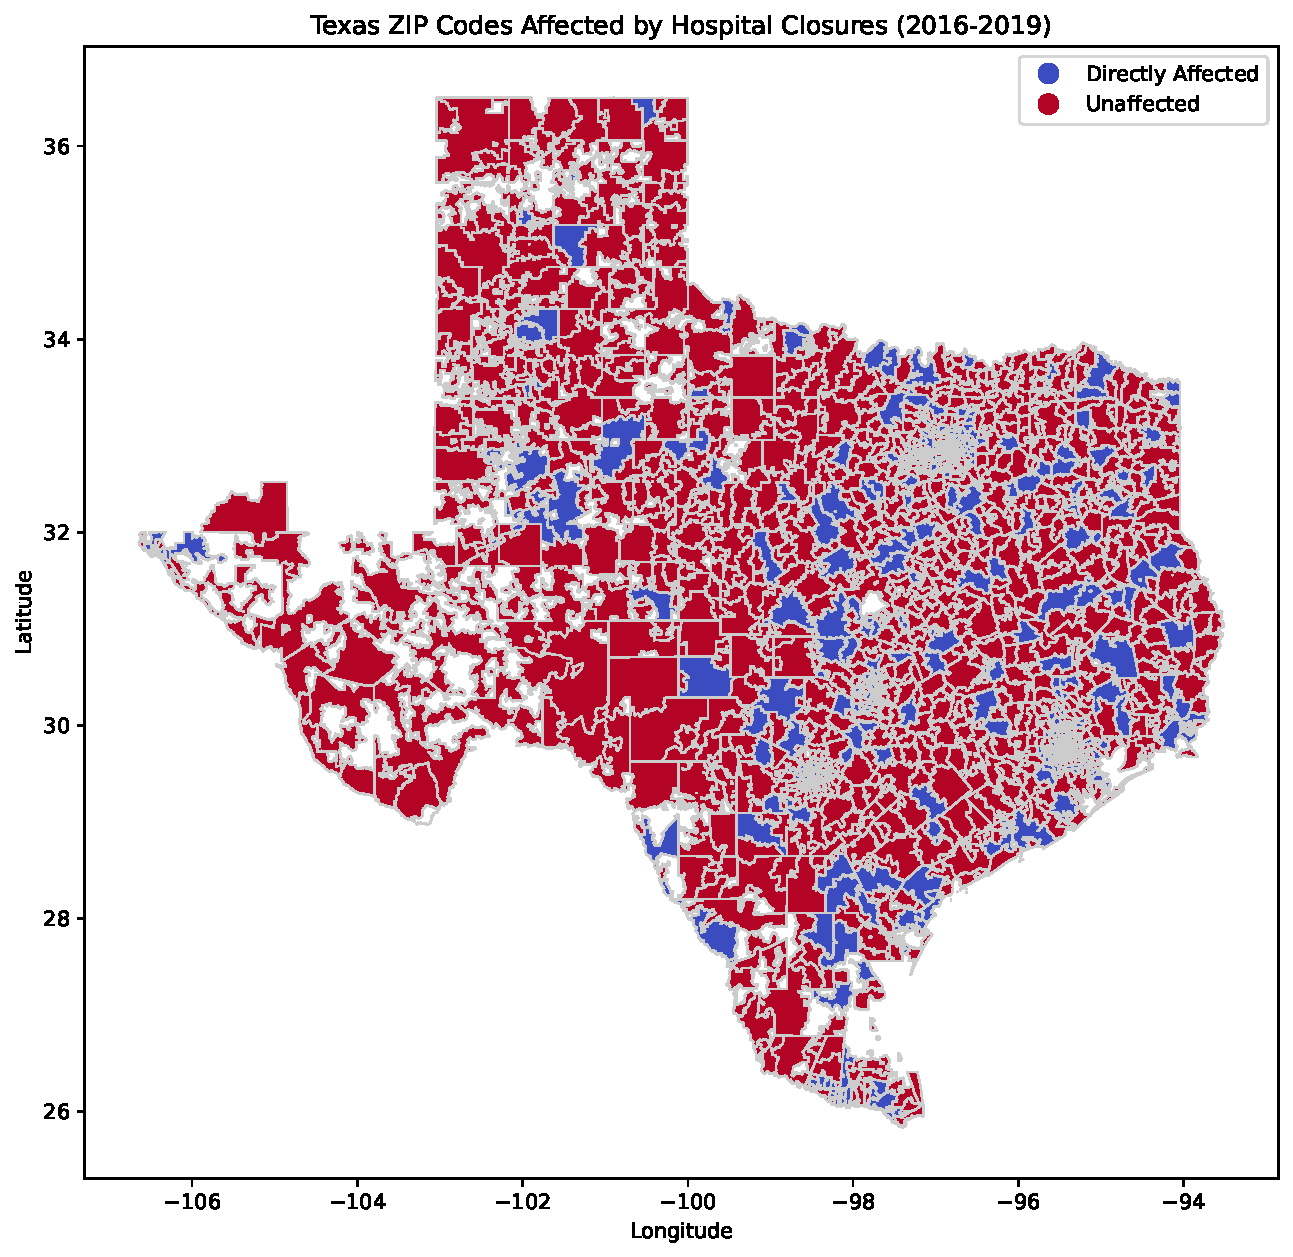
\includegraphics[keepaspectratio]{pset4_template_files/figure-pdf/cell-30-output-1.pdf}}

\subsection{Reflecting on the exercise (10
pts)}\label{reflecting-on-the-exercise-10-pts}

\begin{enumerate}
\def\labelenumi{\arabic{enumi}.}
\item
  Hospitals may close briefly for renovations or disasters, which the
  method might mistake as permanent closures. Mergers, ownership
  changes, or new CMS numbers could be falsely flagged as closures.
  There also might be data larges that there are delayed or incomplete
  updates that can misrepresent a facility's status. I could think of an
  improvement that uses cross-reference with multiple sources, which
  verifies closures by checking other datasets like state health
  departments or news reports. We could also track service types for
  changing services instead of truly closer.
\item
  The current method is to determine the closure rate by checking
  whether the hospitals listed as ``active'' in 2016 remained active or
  disappeared in subsequent years. The method adjusts for closures due
  to mergers by deleting hospitals in postal code areas where the number
  of active hospitals has not decreased. However, if a hospital closes
  and reopens in a neighboring postal code area under a new
  certification, the method may misidentify the closure. Furthermore,
  the method does not take population size into account, so the handling
  of closures is the same in areas with high and low population density.
  Some improvements can be made, such as weighting closures based on the
  population affected by the postal code area to better understand their
  impact, or checking whether the hospital reopens in a neighboring
  postal code area within a shorter distance, which may indicate a
  hospital relocation rather than a true closure.
\end{enumerate}




\end{document}
